\documentclass[a4paper]{article}
\usepackage[utf8]{inputenc}
\usepackage{setspace}
\usepackage{hhline}
\usepackage[document]{ragged2e}
\usepackage{lipsum}
\usepackage{multirow}
\usepackage{multicol}

% Margins for document
\usepackage[left=1.5in, right=1.25in , top=1in, bottom=1in]{geometry}

% using package for TU logo(png)
\usepackage{graphicx}
\graphicspath{ {../resources/images/}}


\setstretch{1.5}
\begin{document}


%% Front Cover %%
\newpage{

	% Latex code for Front Cover

	\pagenumbering{gobble}
	\begin{center}

		
\includegraphics[width=4cm, height=4.3cm]{"../../resources/images/proposal/proposal-tu-logo.png"} \\

		\vspace{5pt}

		\Large{
			\textbf{
				Tribhuvan University \\
				IOE, Pulchowk Campus \\
				Department of Electronics and Computer Engineering \\
			}

			\vspace{10pt}
		}
		% Three vertical lines

		\rule[-80pt]{1pt}{105pt}
		\hspace{20pt}
		\rule[-100pt]{1pt}{150pt}
		\hspace{20pt}
		\rule[-80pt]{1pt}{105pt}

		\vspace{20pt}
		OBJECT ORIENTED PROGRAMMING \\
		PROJECT PROPOSAL\\
		on \\

		\textbf{
			A PHONE CALL \\
			\vspace{20pt}
		}
		\vspace{30pt}

		\begin{multicols}{2}

			\begin{flushleft}
				\section*{Submitted By:}
				Saurav Kumar Mahato\\
				(077BCT079)\\

				Susheel Thapa\\
				(077BCT090)
			\end{flushleft}

			\columnbreak

			\begin{flushright}
				\section*{Submitted To:}
				Department of Electronics\\
				and      \\
				Computer Engineering
			\end{flushright}

		\end{multicols}
	\end{center}

}

%% Acknowledgement %%
\newpage{

	% Latex Code for Acknowledgement

	\setlength{\parindent}{0pt}
	\begin{center}
		\textbf{ {\section*{\huge {Acknowledgement}}}}
	\end{center}

	%%vertical spacing
	\vspace{30pt}

	\Large{

		\justify First of all we would like to thank to our OOP instructor Daya Sagar Baral , Lokh Nath Regmi and Shanti Tamang we helped us
		to learn OOP in C++. Along with learning they provided us the opportunity to apply the concept of OOP to manage our project and use its feacture like  encapsulation, abstraction, inheritance and polymorphism.

		\justify \noindent Would also like to thank whole team of Deapartment of Electronics and Computer Engineering to provide us the
		opportunity to expose our skills and express our learning throught projects.

		\justify \noindent Thanks to all our seniors as well who directly or indirectly help us through the learning process and made our journey easy through different session and workshops.

		\justify \noindent Finally, thanks to all our friends and classmates who helped in discussing different idea and workflow of the project along with providing good suggestions.

	}
}

%% Table of contents %%
\newpage
{

	% Latex code for Table of contents

	\begin{center}
		\textbf{ \huge{Table of contents}}
		\vspace{30pt}
	\end{center}


	\vspace{20pt}

	\Large{

		\textbf{1. Introduction	.........................................................1 \\ }
		\vspace{20pt}
		\textbf{2. Objectives  ............................................................2\\}
		\vspace{20pt}
		\textbf{3. Existing System ...................................................3\\}
		\vspace{20pt}
		\textbf{4. Proposed System \\}
		\vspace{20pt}
		\hspace{15pt}\textbf{4.1 Introduction ....................................................4 \\}
		\vspace{20pt}
		\hspace{15pt}\textbf{4.2 System Block Diagram ....................................4 \\}
		\vspace{20pt}
		\textbf{5. Methodology \\}
		\vspace{20pt}
		\hspace{15pt}\textbf{5.1 Tool we will used .............................................5 \\}
		\vspace{20pt}
		\hspace{15pt}\textbf{5.2 Approach to the project ..................................6  \\}
		\vspace{20pt}
		\textbf{6. Project Scope .......................................................7 \\}
		\vspace{20pt}
		\textbf{7. Project Schedule ..................................................8}
		\vspace{20pt}

	}

}



%% Introduction %%
\newpage{

	% Latex Code for Introduction

	\pagenumbering{arabic}
	\vspace{30pt}

	\begin{center}

		\textbf{ \huge{Introduction}}

	\end{center}

	\vspace{30pt}

	\Large{

		\justify Our project (A Phone Call) was initiated with the aim to demostrate how the call get established between two client in the real world and what actually is happening behind the scene.

		\vspace{10pt}

		\justify The key objectives of this project is to focus over two client who will be trying to call each other. And middle person(server) will be routing the call to the designated person after, it has successfully decoded the signal that has been passed to it by one of its client. Moreover, we will also focus over the storing data like who have called to whom and when did they have so that we can display a call log on our client side.


		\vspace{10pt}

		\justify It doesn't indent to include all the feature that is found in our call app of our phone but we will to try make the call app as real as possible.
		Also, we aren't going for the communication over the voice call as it is beyond the scope of this project.

		\vspace{10pt}

		\justify At last,\textbf{A Phone Call} focus over how a call get connected between two user when one user calls another user and the hidden detail of what is happening in background. Also, it will include some feature of the Our Calling app to make is a bit realistic.

	}

}

%% Objectives %%
\newpage{

	% Latex Code for Objectives

	\begin{center}

		\textbf{ \huge{Objectives}}

	\end{center}

	\vspace{20pt}

	\LARGE{
		Following are the objective of our OOPs project:
	}

	\vspace{10pt}

	\Large{
		\begin{enumerate}
			\item To learn Object Oriented Programming paradigm.
			\item To learn Simple Media Direct Layer(\textit{ a  library that provide 2D graphics.})
			\item {Understanding how does client and server communicate with each other.}
			\item Enhancing concept over interaction with database via C++ program
			\item Understanding how does A Phone Call work in real life
			\item Understanding the concept behind the signal processing that is used in real world by many network provider(\textit{Dual Tone Multi Frequency})
			\item Understanding the special feature C++ like

			      \begin{enumerate}
				      \item Function and Operator Overloading
				      \item Virtual Function
				      \item Stream Class
				      \item Exception Handling
				      \item Standard Template library(\textit{STL})
			      \end{enumerate}

			\item  To learn how to collaborate with each other in a project.

		\end{enumerate}
	}
}

%% Existing System %%
\newpage{

	% Latex Code for Existing System

	\begin{center}

		\textbf{ \huge{Existing System}}
		\vspace{10pt}
		\Large{

			\justify{
				\textbf{A Phone Call} is simple to demonstrate how does the call get establish between any two user who are connected in any network.


				\noindent \justify The most common example of existing in the real world are network provider like Nepal Telecom , Ncell. What mainly happen is that a person calls another person from his phone by dialing number and call the call gets conneted to the destination after the server ( NCELL OR NTC as instance) does its work.
				The calling service provider acts as the bridge between two clients and allows to share information with each other.

				\noindent \justify This is what all the phone or sim company does and charges money. So, eventually in context of Nepal, the best example of existing system for this project can be NCELL and NTC.
			}
		}
	\end{center}

}

%% Proposed System %%
\newpage{

	% Latex Code for Proposed System

	\setlength{\parindent}{0pt}
	\begin{center}
		{\section*{\huge {Proposed System}}}
	\end{center}


	\vspace{20pt}


	\Large{
		\subsection*{\Large{Introduction}}
		\Large{

			\justify{
				CallApp is a mobile app offering caller ID, call blocking and call recording. It gives background information about the entities behind incoming or outgoing calls by utilizing the user community-generated content and social networking services.

				\vspace{10pt}

				\noindent	And Phone Call is subset of CallApp which  bascially demonstrate calling features, call logs, decoding of signal, receiving the phone call of the CallApp.
			}

		}

		\vspace{20pt}

		\subsection*{\Large{System Block Diagram}}

		\begin{center}

			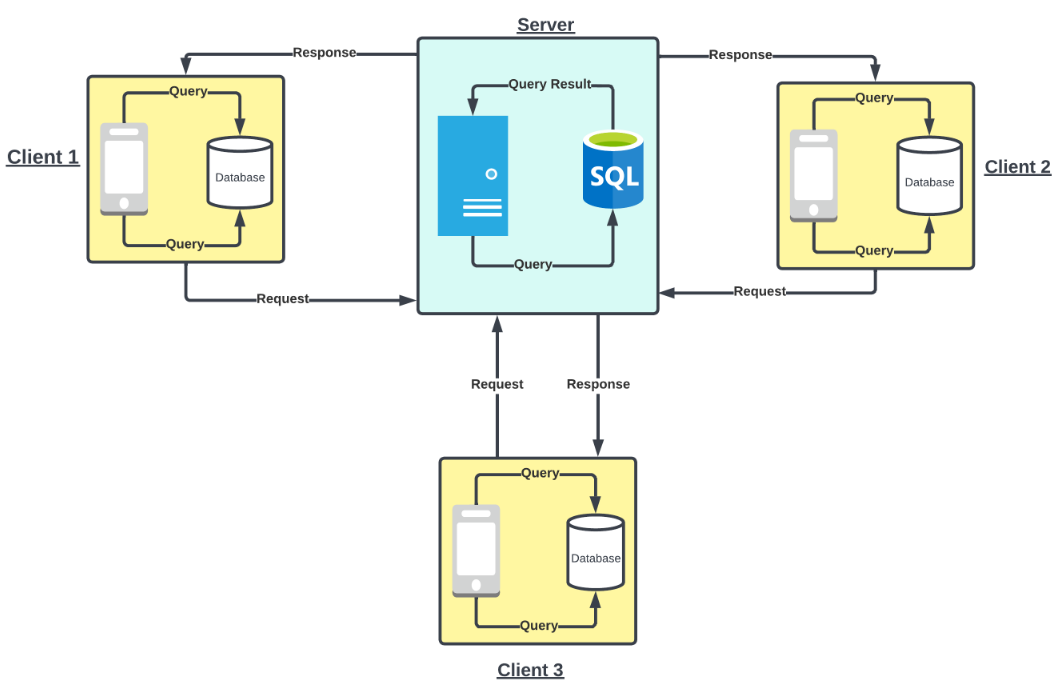
\includegraphics[width=450px, height=300px]{
				"../../resources/images/proposal/proposal-block_diagram_opaque.png"}


		\end{center}


	}

}

%% Methodology %%
\newpage{

	% Latex Code for Methodology

	\begin{center}

		\textbf{ \huge{Methodology}}

	\end{center}

	\section*{Tool we will be using}

	\Large{
		\begin{enumerate}
			\item  \textbf{\textit{Visual Studio Code}} as our code editor.
			\item  \textbf{\textit{g++}} as our compiler to compile our project file.
			\item \textbf{\textit{maraidbcpp connector}} to connect with our mariadb database.

			\item \textbf{\textit{sqlite3 header file}} to connect with our sqllite3 database.
			\item \textit{\textbf{socket programming}} to create our client and server.
			\item \textbf{\textit{SDL2}} to create GUI interface on Client side.
			\item \textbf{\textit{Git}} as our local version control system and \textbf{\textit{Github}} as our centralized version control system.
			\item \textbf{{\LaTeX{}}} as our Document Preparation system for proposal and project report.
			\item \textbf{\textit{Linux}} as our working Operating System


		\end{enumerate}

	}

	\newpage{
		\section*{Approach to Project}

		\Large{
			\begin{enumerate}
				\item Since our project is based over networking and database so we need to do two things at first i.e Building up client and server and Interaction with database.

				\item After we have setup client/server and Interaction with database we will be working into the GUI part of the project(mostly client side)  as we will be using terminal console to display the mesage from the sever.


				\item Then we will integrated our GUI with the client and try to setup the connection with the server.
				\item After we become successful over one client then we will go for setup three client.

				\item Then before heading to the phone call we wil first try messging feature between client i.e we will try to message client 2 form client 1 and vice versa.

				\item Once it is successful we wiil implement that for the call.

				\item After successful implementaation of calling feature. We will integrated all those with the database so that we can display the call logs to the client.
			\end{enumerate}
		}

	}
}

%% Project Scope %%
\newpage{

	% Latex Code for Project Scope

	\setlength{\parindent}{0pt}

	\begin{center}
		\textbf{ {\section*{\huge {Project Scope}}}}
	\end{center}

	\vspace{30pt}

	\setlength{\parindent}{0pt}

	\Large{
		\justify The main idea of this project is to create the MVP( Minimum Viable Product) to show the real life events happening in our daily life. All we need was some databases to store the information related to call logs with some graphics, client-server model and of course OOP. One will see some interface similar to their phone dial pad and will be able to type number and listen the specific sound of the number after pressing it. After dialing the number, called window ( like in our daily life when call comes ) will appear on the screen.



		\justify{
			These are the outcomes of this project in real world.

			\begin {enumerate}
			\item It aims over how things are working behind the scene while calling each other and how does they know we are calling whom.
			\item It aims to provide a real time simulation of Calling App that exist in almost all mobile phones.
			\item It will be able to make people understand why it say \textit{Tapaile samparka garna khojeko manche bessta xa, tapaile samparka garna khojeko number switch off xa} and many other.
			\item Also it will explain why there is system of ringtone when we call other person.
			\end{enumerate}
		}
	}
}


%% Project Schedule %%
\newpage{

	% Latex Code for Project Schedule

	\setlength{\parindent}{0pt}
	\begin{center}
		\textbf{ {\section*{\huge {Project Schedule}}}}
	\end{center}

	\vspace{30pt}
	\setlength{\parindent}{0pt}
	\Large
	{
		\justify The whole project can be divided into two part client side and sever side. Client side will take more time as it will contain the graphic part or visible part.
		As discussed in the methodology, the project will all together take around 20 to 30 days.

		\justify {All the phases in making this project and their time requirement is given below in table:} \\

		\begin{center}
			\begin{tabular}{||l|c||}
				\hline
				\hspace{50pt} Phases:     & Days Required: \\
				\hline
				Project Brainstorming     & 2 days         \\
				Algorithm and Flowchart   & 3 days         \\
				Server side programming   & 4 days         \\
				Client side programming   & 7 days         \\
				Linking server and client & 3 days         \\
				Testing and Debugging     & 3 days         \\
				Deployment(GitHub)        & 2 days         \\

				\hline
			\end{tabular}

		\end{center}
		All the number of days given above is approximate days estimated.

	}

}
\end{document}
